\chapter{M\'odulo de Clientes}

\section{Descripci\'on General}

El m\'odulo de clientes gestiona los due\~nos de mascotas registrados en
el sistema. Proporciona operaciones CRUD completas con b\'usqueda, filtrado
por cl\'{\i}nica y notificaciones autom\'aticas.

\section{Server Actions}

El archivo \texttt{lib/actions/clients.ts} implementa 5 server actions:

\begin{lstlisting}[style=typescript, caption=Server actions de clientes]
'use server';

import { db, schema } from '@vetrinaria/db';
import { eq, and } from 'drizzle-orm';
import { revalidatePath } from 'next/cache';
import { z } from 'zod';
import { createNotification } from './notifications';
import { getCurrentClinicId } from '@/lib/clinic';

const clientSchema = z.object({
  name: z.string().min(1, 'El nombre es obligatorio'),
  email: z.string().email('Email invalido').optional().or(z.literal('')),
  phone: z.string().min(1, 'El telefono es obligatorio'),
  address: z.string().optional(),
  emergencyContact: z.string().optional(),
  notes: z.string().optional(),
});

export type ClientInput = z.infer<typeof clientSchema>;
\end{lstlisting}

\subsection{Patrones de Implementaci\'on}

\begin{itemize}[leftmargin=*]
    \item \textbf{Validaci\'on con Zod:} \texttt{clientSchema.parse(data)}
          lanza error si los datos no cumplen el esquema.
    \item \textbf{Clinic-scoped:} Todas las consultas usan
          \texttt{getCurrentClinicId()} para filtrar por cl\'{\i}nica.
    \item \textbf{B\'usqueda h\'{\i}brida:} La funci\'on \texttt{getClients}
          filtra en base de datos por cl\'{\i}nica y luego aplica un filtro
          adicional en JavaScript para b\'usqueda por texto parcial en
          nombre, email y tel\'efono.
    \item \textbf{Notificaciones:} Al crear un cliente, se notifica a todos
          los administradores de la misma cl\'{\i}nica.
    \item \textbf{Revalidaci\'on:} \texttt{revalidatePath} invalida el
          cach\'e de las rutas afectadas.
\end{itemize}

\subsection{getClients --- Listado con Búsqueda}

\begin{lstlisting}[style=typescript, caption=Funcion getClients]
export async function getClients(search?: string) {
  const clinicId = await getCurrentClinicId();
  const clinicFilter = eq(schema.clients.clinicId, clinicId);

  const rows = await db
    .select()
    .from(schema.clients)
    .where(
      search
        ? and(clinicFilter, eq(schema.clients.active, true))
        : clinicFilter,
    )
    .orderBy(schema.clients.name);

  if (search) {
    return rows.filter(
      (c) =>
        c.name.toLowerCase().includes(search.toLowerCase()) ||
        c.email?.toLowerCase().includes(search.toLowerCase()) ||
        c.phone.includes(search),
    );
  }

  return rows;
}
\end{lstlisting}

\section{P\'aginas}

\subsection{Listado (/clients)}

\begin{itemize}[leftmargin=*]
    \item Tabla responsiva con columnas: nombre, email, tel\'efono, acciones.
    \item Barra de b\'usqueda con par\'ametro \texttt{?q=} en la URL.
    \item Bot\'on ``Nuevo Cliente'' que enlaza a \texttt{/clients/new}.
    \item Cada fila tiene enlaces a detalle y edici\'on.
\end{itemize}

\subsection{Creaci\'on (/clients/new)}

\begin{itemize}[leftmargin=*]
    \item Formulario con campos: nombre (obligatorio), email, tel\'efono
          (obligatorio), direcci\'on, contacto de emergencia, notas.
    \item Validaci\'on del lado del servidor con Zod.
    \item Manejo de estado de carga y errores.
\end{itemize}

\subsection{Detalle (/clients/[id])}

\begin{itemize}[leftmargin=*]
    \item Informaci\'on de contacto completa.
    \item Secci\'on de mascotas registradas del cliente (integrada con
          el m\'odulo de pacientes).
    *timestamps de creaci\'on y actualizaci\'on.
\end{itemize}

\subsection{Edici\'on (/clients/[id]/edit)}

\begin{itemize}[leftmargin=*]
    \item Formulario precargado con los datos existentes.
    \item Mismo componente \texttt{ClientForm} reutilizable.
\end{itemize}

\section{Componente Reutilizable}

El \texttt{ClientForm} es un componente cliente (\texttt{'use client'}) que:

\begin{itemize}[leftmargin=*]
    \item Recibe \texttt{defaultValues} y \texttt{onSubmit} como props.
    \item Usa \texttt{useState} para manejo de carga y errores.
    \item Procesa datos con \texttt{FormData} nativo del navegador.
    \item Muestra bot\'on de env\'{\i}o con estado de carga.
\end{itemize}

\section{API Routes}

\begin{lstlisting}[style=typescript, caption=API de listado de clientes para selects]
// api/clients/list/route.ts
export async function GET() {
  const clients = await db
    .select({ id: schema.clients.id, name: schema.clients.name })
    .from(schema.clients)
    .where(eq(schema.clients.active, true))
    .orderBy(schema.clients.name);

  return Response.json(clients);
}
\end{lstlisting}

Esta API es consumida por otros formularios (citas, facturas) para cargar
selectores de clientes.

\begin{figure}[H]
    \centering
    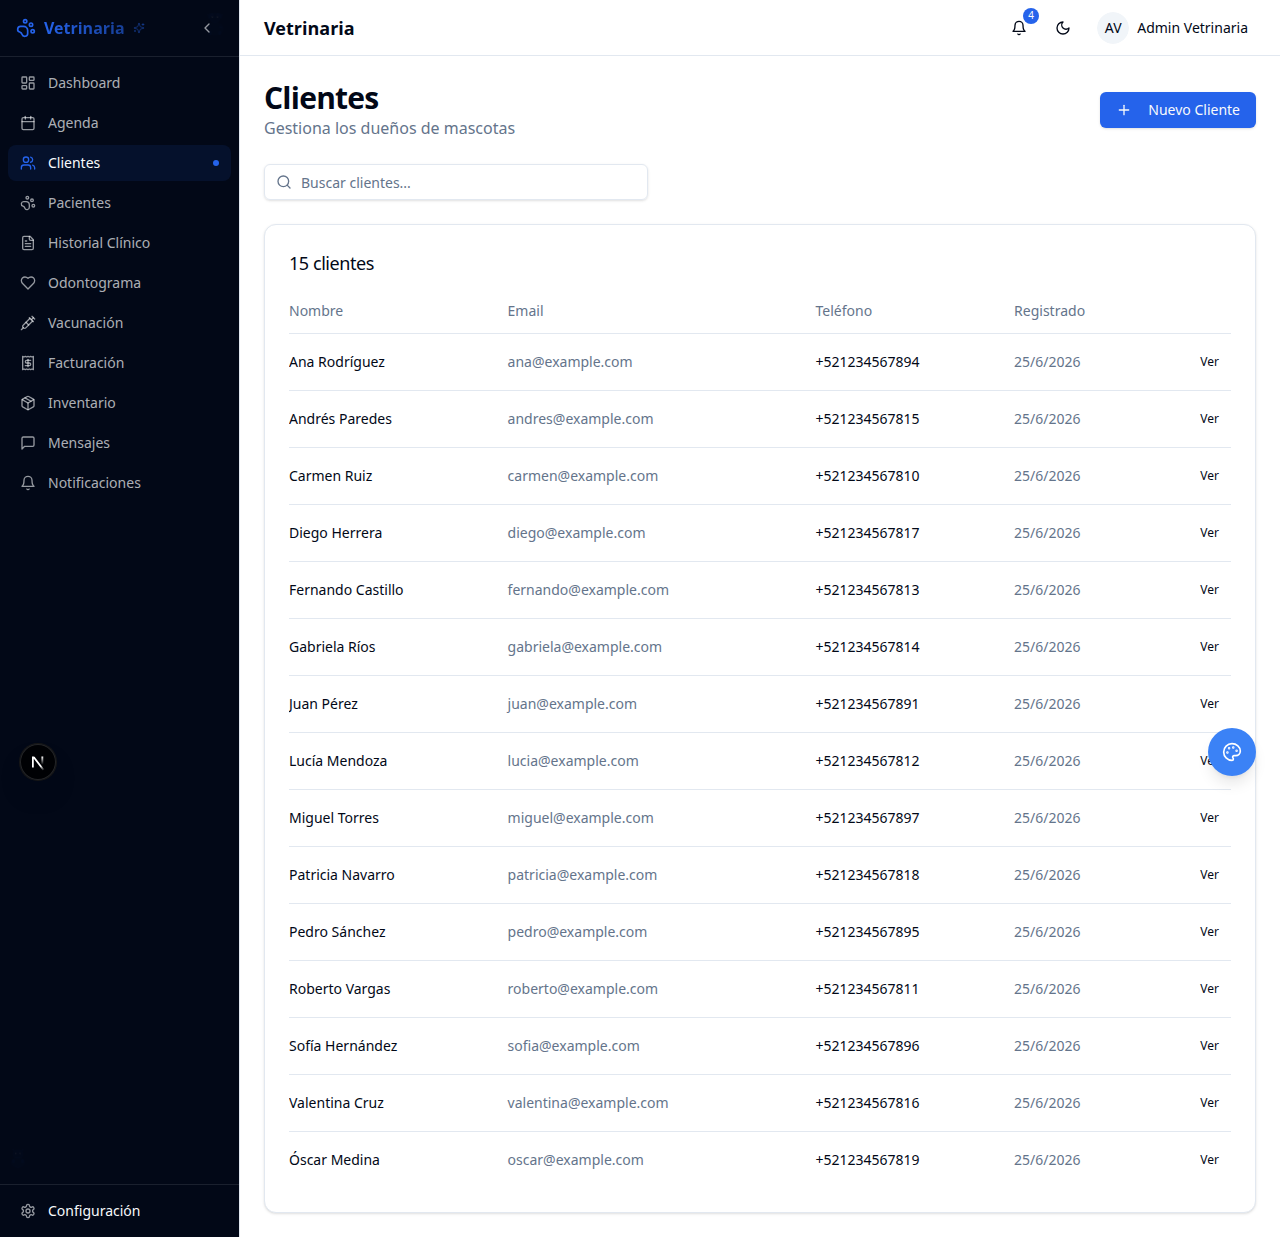
\includegraphics[width=\textwidth]{img/vet-clients.png}
    \caption{Listado de clientes con busqueda y tabla responsiva}
    \label{fig:clientes}
\end{figure}
